\documentclass{article}

\usepackage[utf8]{inputenc}
\usepackage[margin=1in]{geometry}
\usepackage{hyperref}
\usepackage{graphicx}
\usepackage{float}
\usepackage{caption}
\usepackage{subcaption}
\usepackage{titlesec}

\setcounter{secnumdepth}{4}
\setcounter{tocdepth}{4}
\titleformat{\paragraph}
{\normalfont\normalsize\bfseries}{\theparagraph}{1em}{}
\titlespacing*{\paragraph}
%{0pt}{3.25ex plus 1ex minus .2ex}{1.5ex plus .2ex}
{0pt}{0.0ex plus 1ex minus .2ex}{1.0ex plus .2ex}

\newcommand{\name}{ECW\ }
\newcommand{\nameNospace}{ECW}
\newcommand{\namep}{ECW.}

\renewcommand{\labelenumii}{\theenumii}
\renewcommand{\theenumii}{\theenumi.\arabic{enumii}}
\renewcommand{\theenumiii}{\theenumii.\arabic{enumiii}}

\usepackage{fancyhdr}
\pagestyle{fancy}

\lhead{ Responsible: Alexander Ekman \& Linnea Johnsson \\ Date: \today}  \rhead{Document number: PUSS21411 \\ Version: 1.3}
\renewcommand{\headrulewidth}{0.5pt} 


 \title{SDP - Software Development Plan}
 \author{Team 1 - ETSN05}

\begin{document}
\date{}
\maketitle
\thispagestyle{fancy}
\newpage

\section*{Revision History}
\begin{table}[h]
    \centering
    \begin{tabular}{|l|l|p{55mm}|p{35mm}|}
    \hline
    Date & Version & Description & Author \\ 
    \hline\hline 
    2021-09-14 & 1.0 & First draft and outlines of all sections & Linnea Johnsson \\
    \hline
    2021-09-25 & 1.1 & Updated according to review comments & Linnea Johnsson \\ 
    \hline
    2021-09-26 & 1.2 & Updated time allocation and Gantt chars & Linnea Johnsson  \\ 
    \hline
    2021-09-27 & 1.3 & Updated risks based on team feedback & Linnea Johnsson \& David Ravanelli \\ 
    \hline
    \end{tabular}
    \label{tab:history}
\end{table}
\newpage
 
\section*{Referenced Documents}\label{refdoc}
\begin{enumerate}
    \item Programvaruutveckling för Stora System - Projekthandledning 2021 (PH)
    \item Product Requirements Document - PUSS21412 (PRD)
    \item Software Product Features Backlog(SPF) - PUSS21413
    \item Sprint log/plan (SP) - PUSS21414
    \item Software Top Level Design Document (STLDD) - PUSS21415
    \item Software Detailed Design Document (SDD) - PUSS21416
    \item Software Verification and Validation Report (SVVR) - PUSS21417
    \item System Specification Document (SSD) - PUSS21418
    \item Project Final Report (PFR) - PUSS21419

\end{enumerate}
\newpage

\tableofcontents
\newpage

\section{Introduction}
This Software Development Plan (SDP) details the development plan produced for the development of the web-app based carpool service called ETSN05\_PG1 Carpool Webb-app (ECW). The description of this product can be found in the PH document chapter 9. Furthermore, the SDP derives mostly from the PH and includes the process model with the project's different phases and their corresponding time-estimates and major events, and the tailoring of the project. The SDP also includes a description of the project's organisation, time plan, configuration handling, and quality review, as well as a a risk analysis of the project. 

\section{Project Organisation}
The project is organized into a Project Group (PG), Developing Group (DG), and a System Group (SG). The PG consists of the Project Owners (PO) and Scrum Master(SM), the DG consists of developers and the architects, and the SG consists only of the architects. Within the DG there are different areas of responsibilities. There are mainly four areas of responsibilities that corresponds to three different groups, and one sole role. There is the Algorithms Group (AG), the Frontend Group (FG), and the Backend Group(BG). There is also one role responsible for testing (TR). 

Besides the above mentioned internal actors the project has an External Group (EG), which include a section chief, a customer, a reviewer, and three different experts roles. The experts have different areas of expertise. There is one requirement expert, one test expert, and one design expert.

\subsection{Project team members}
The project's team member and their corresponding roles can be seen in table \ref{team}. All internal team members are enrolled in the course ETSN05 and participating in the project for educational purposes. The members have been given their different groups and roles based on interests and experience. The external team members are educational staff members in the course.
\begin{table}[h]
    \centering
    \begin{tabular}{|c|c|c|}
    \hline
        Group & Name & Role \\
        \hline \hline
        PG & Alexander Ekman & PO \\ 
        & Linnea Johnsson & PO \\
        & David Ravanelli & SM \\
        \hline
        AG & Max Fogwall & Architect \& TR \\
        & Emil Friberg & Developer \\
        & Gustav Broman & Developer \\
        \hline
        FG & Erik Kullberg & Architect \\
        & Axel Domell & Developer\\ 
        & Erik Busk & Developer \\
        & Johannes Bastmark & Developer\\
        \hline
        BG & Anton Håkansson & Developer\\
        & Elsa Lindhé & Developer\\
        & Eric Schyllert  & Developer\\
        \hline
        EG & Alma Orucevic-Alagic & Customer, Chief \& Reviewer \\
        & Rasmus Ros & Design expert \\
        & Sergio Rico & Requirements \& Test Expert \\
        \hline
    \end{tabular}
    \caption{The ECW project's team members}
    \label{team}
\end{table}

\section{Process model}
The process model mostly follow the directions from the PH chapter 2. The things that differ, and/or need more explanation, are described below.
\subsection{Phases}
The project is divided into four phases, where the last three are part of sprints. All phases include milestones in the form of documents to produce, deadlines to meet and meeting to have.

The meetings that are held in the different phases include the Sprint Planning Meeting (SPM), the Daily Stand-up Meetings (DSM), the Reflection Meeting(RefM), the Review Meetings(RevM), Internal Project Meetings(IPM), and External Project Meetings (EPM). The latter refer to meetings between the project's internal groups having meetings with the project's external actors. The person responsible for the different meetings is presented in table \ref{tab:meetings}. Being responsible for a meeting includes calling it and assigning someone or oneself as responsible of  note taking and action list creation. One exception is RevMs, where by default the PG has this responsibility. Another exception is in EPMs, where someone of the internal actors in order of first PG, then SG and lastly DG has this responsibility.

RefMs and SPMs will be held in connection to either Mondays
' or Fridays' DSMs in order to ensure high attendance. These weekdays' DSM are held over Zoom in order to better connect to the team and more easily raise issues or concerns. The rest of the DSMs are  held on a designated Slack channel in order to accommodate the team members conflicting schedules. 

The sprint phases requires time for development of the ECW, but all phases includes some level of mandatory coursework that require time from the project members. The time allocation will be further explained in section Time Plan. 

\begin{table}[H]
    \centering
    \begin{tabular}{|c|c|}
    \hline
        Meeting & Head responsible \\
        \hline \hline
        SPM & PG \\
        \hline
        DSM & SM \\
        \hline
        RefM & SM \\
        \hline
        RevM & Reviewer \& PG \\
        \hline
        IPM & PG, DG or SG  \\
        \hline
        EPM & Anybody \\
        \hline
    \end{tabular}
    \caption{The different meetings that are held within the project and role that is head responsible for the meetings}
    \label{tab:meetings}
\end{table}

\subsubsection{Phase 1}
In table \ref{tab:phase1} the major events from the first phase are listed in order to create an easily accessible overview. This phase focuses on specification.
\begin{table}[H]
    \centering
    \begin{tabular}{|c|c|c|}
    \hline
        Event & Deadline & Responsible/Attending \\
        \hline \hline
        SDP & 2021-09-15 & PO/- \\
        \hline
        PRD & 2021-09-15 & PO/- \\
        \hline
        SPM1 & 2021-09-10 & PG/All \\
        \hline
        SPF1 & 2021-09-10 & PO/- \\
        \hline
        SP1 & 2021-09-10 & SG \& DG/- \\
        \hline
        RevM 1 & 2021-09-17 & PG/All \\
        \hline
    \end{tabular}
    \caption{The major events occurring in phase 1}
    \label{tab:phase1}
\end{table}

\subsubsection{Phase 2}
Table \ref{tab:phase2} shows the seconds phase's main activities. This phase focuses on the first sprint and high-level design.
\begin{table}[H]
    \centering
    \begin{tabular}{|c|c|c|}
    \hline
        Event & Deadline & Responsible/Attending \\
        \hline \hline
        Sprint 1 & 2021-09-26 & DG \& SG/- \\
        \hline
        RefM & 2021-09-24 & SM/All \\
        \hline
        DSM & - & SM/ SG \& DG \\
        \hline
        STLD & 2021-09-29 & SG/- \\
        \hline
        SPM2 & 2021-09-24 & PG/All \\
        \hline
        SPF2 & 2021-09-14 & PO/- \\
        \hline
        SP2 & 2021-09-14 & SG \& DG/- \\
        \hline
        RevM 2 & 2021-10-01 & PG/All \\
        \hline
    \end{tabular}
    \caption{The major events occurring in phase 2}
    \label{tab:phase2}
\end{table}

\subsubsection{Phase 3}
The thirds phase's major event are included in table \ref{tab:phase3}. The third phase focuses on sprint 2 and low-level design. 
\begin{table}[H]
    \centering
    \begin{tabular}{|c|c|c|}
    \hline
        Event & Deadline & Responsible/Attending \\
        \hline \hline
        Sprint 2 & 2021-10-10 & DG \& SG/- \\
        \hline
        RefM & 2021-10-08 & SM/All \\
        \hline
        DSM & - & SM/ SG \& DG \\
        \hline
        SDD & 2021-10-13 & DG/- \\
        \hline
        SPM3 & 2021-10-08 & PG/All \\
        \hline
        SPF3 & 2021-10-08 & PO/- \\
        \hline
        SP3 & 2021-10-08 & SG \& DG/- \\
        \hline
        RevM 3 (informal) & 2021-10-15 & PG/All \\
        \hline
    \end{tabular}
    \caption{The major events occurring in phase 3}
    \label{tab:phase3}
\end{table}

\subsubsection{Phase 4}
The last phase's major events can be viewed in table \ref{tab:phase4}, including and ending with the final review. The last phase focuses on sprint 3, integration, system testing as well as checking, and producing, the last documentation.
\begin{table}[H]
    \centering
    \begin{tabular}{|c|c|c|}
    \hline
        Event & Deadline & Responsible/Attending \\
        \hline \hline
        Sprint 3 & 2021-10-22 & DG \& SG/- \\
        \hline
        RefM & 2021-10-22 & SM/All \\
        \hline
        DSM & - & SM/ SG \& DG\\
        \hline
        SVVR & 2021-10-22 & SG \& DG/- \\
        \hline
        SSD & 2021-10-22 & PO/- \\
        \hline
        PFR & 2021-10-22 & PO/- \\
        \hline
        RevM final & 2021-10-22 & PG/All \\
        \hline
    \end{tabular}
    \caption{The major events occurring in phase 4}
    \label{tab:phase4}
\end{table}

\section{Configuration Handling}
This project consists of several documents of different character, varying from source code to text documents such as this. There are two main libraries for the different types of configuration units. The first one is GitLab that contains the project's source code, the backlog, the sprint logs, and the SG's \& DG's drafts of the STLDD, SDD, SVVR, \& SSD. The main text documents such as the SDP, PRD, and PFR are stored in a GitHub repository in phase one and two, with the hope that we can integrate these to GitLab as well.

The configuration units are numbered according to the PH, and a list of the different document numbers can be seen in section Referenced Documents. Baseline versions are created prior to review hand ins.  

\section{Time plan}
The project will run in parallel with other mandatory coursework. Below follows an estimation of the time allocation for the project, as well as Gantt charts for the main activities and the development process. 

\begin{figure}[H]
    \centering
    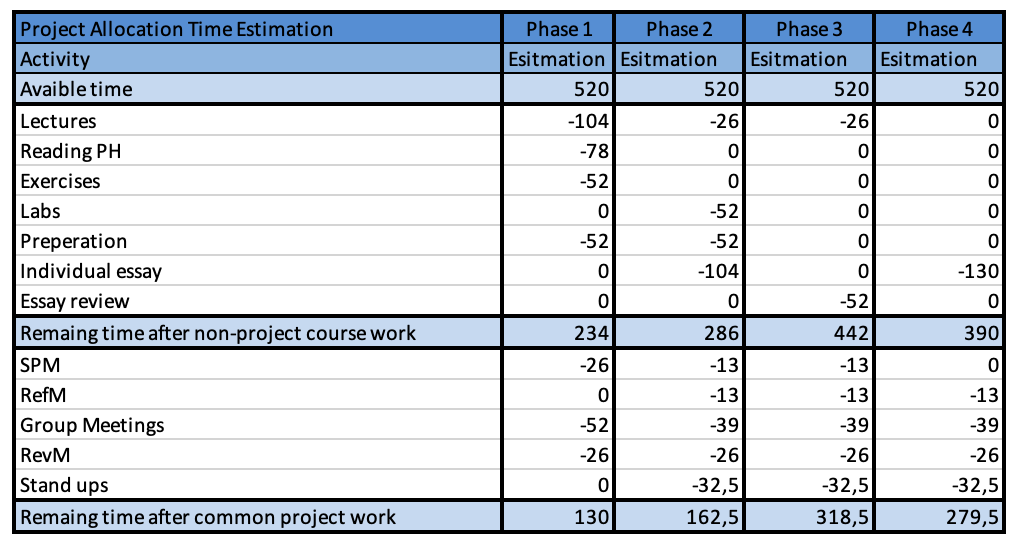
\includegraphics[scale=0.8]{sdpFigures/TimeEstPart1V2.png}
    \caption{Time allocation estimation for the major course- and project events that are mutual for all internal team members. The presented available time is per the entire internal team, i.e. for 13 team members.}
    \label{fig:timeEst1}
\end{figure}

\subsection{Time Allocation Estimation}
In figure \ref{fig:timeEst1} the major course- and project events that are common for the entire project team, with their estimated time allocation needed for them, are presented. The time allocation estimation for the role specific project events are found in figure \ref{fig:timeEst2}. The estimation in figure \ref{fig:timeEst1} takes into account that each team  member has 20 hours per week for the course and that the different phases have a different amount of mandatory course work. The result from figure \ref{fig:timeEst1} is then divided by 13 in figure \ref{fig:timeEst2} in order to represent the remaining time available to allocate per person. This time is to be used in their group role specific tasks. 

The DG is divided into different subgroups, but will work with a hands-on approach. If the FG and BG has a lot to do while the AG does not, the AG members help out where needed. E.g. in the first sprint more focus is put on the front end issues since the AG and BG would need more time to plan and draw out their implementations. When the planning is done, they are to help out with available issues or create new one if needed. 

From figure \ref{fig:timeEst2} it can be extracted that phase three have the most time available for the sprints. A reason for this is that phase one and two has a greater focus on common coursework and on getting started with the project, i.e. figuring out how to correctly formulate and estimate issues and more. While phase four includes more documents needing to be produced, and loose strings needing to be tied up in order to deliver a working system. 

An overhead has also been included, since allocating every possible unit of time does not allow for the flexibility needed in the agile way of working. For the PG this overhead is used to compensate for an uneven workload over the different phases. The PG have more to do in the beginning and end of the project, and a little less in the middle. 

\begin{figure}[h!]
     \centering
     \begin{subfigure}{\textwidth}
         \centering
         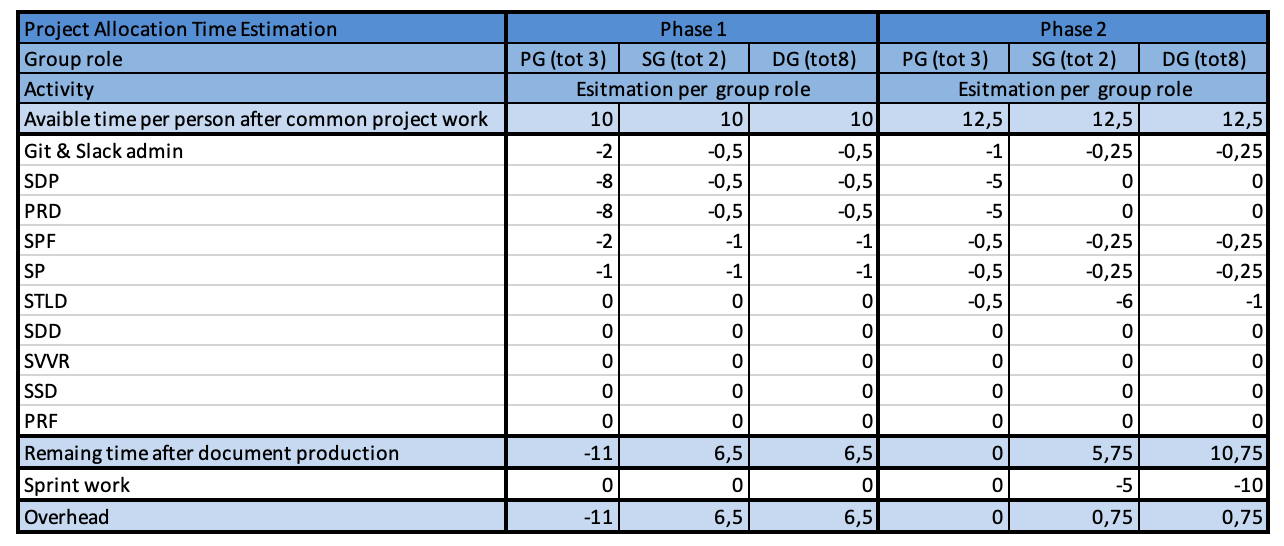
\includegraphics[width=\textwidth]{sdpFigures/TimeEstPart2V2.png}
         \label{fig:y equals x}
     \end{subfigure}
     \hfill
     \begin{subfigure}{\textwidth}
         \centering
         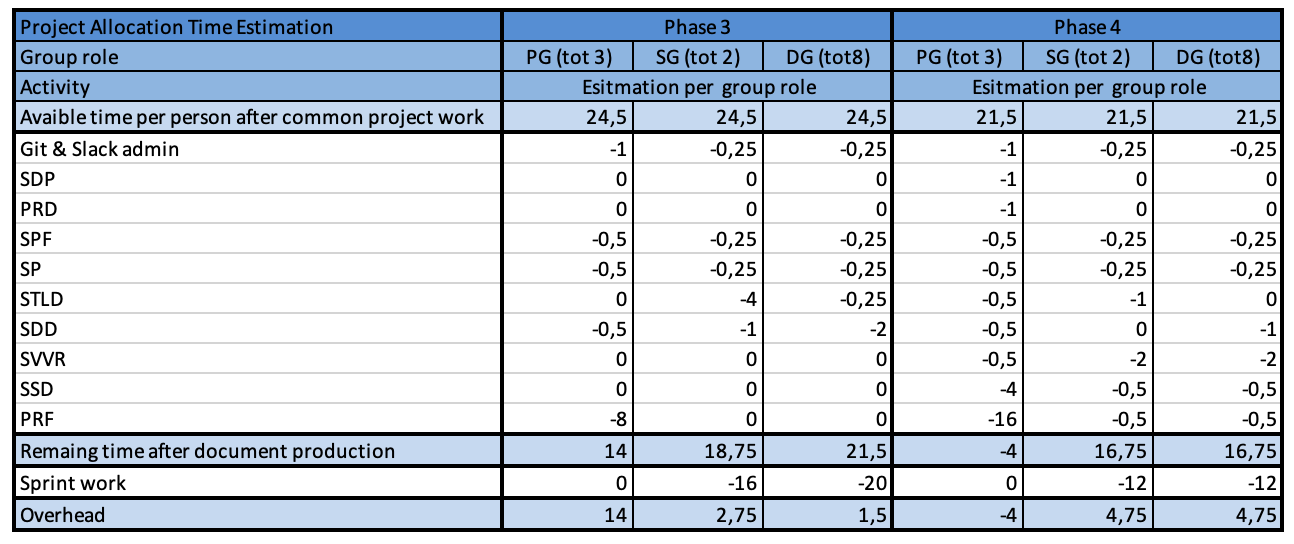
\includegraphics[width=\textwidth]{sdpFigures/TimeEstPart3V2.png}
         \label{fig:five over x}
     \end{subfigure}
        \caption{Time allocation estimation for the major project events per group role and phase. The starting value of available time comes the last row in figure \ref{fig:timeEst1} per phase divided by 13 team members}
        \label{fig:timeEst2}
\end{figure}

\subsection{Gantt Activity chart}
The planning of the main activities of the project in relation to each other, excluding the development of the product, is shown in figure \ref{fig:GantAct}'s Gantt chart.
\begin{figure}[h!]
    \centering
    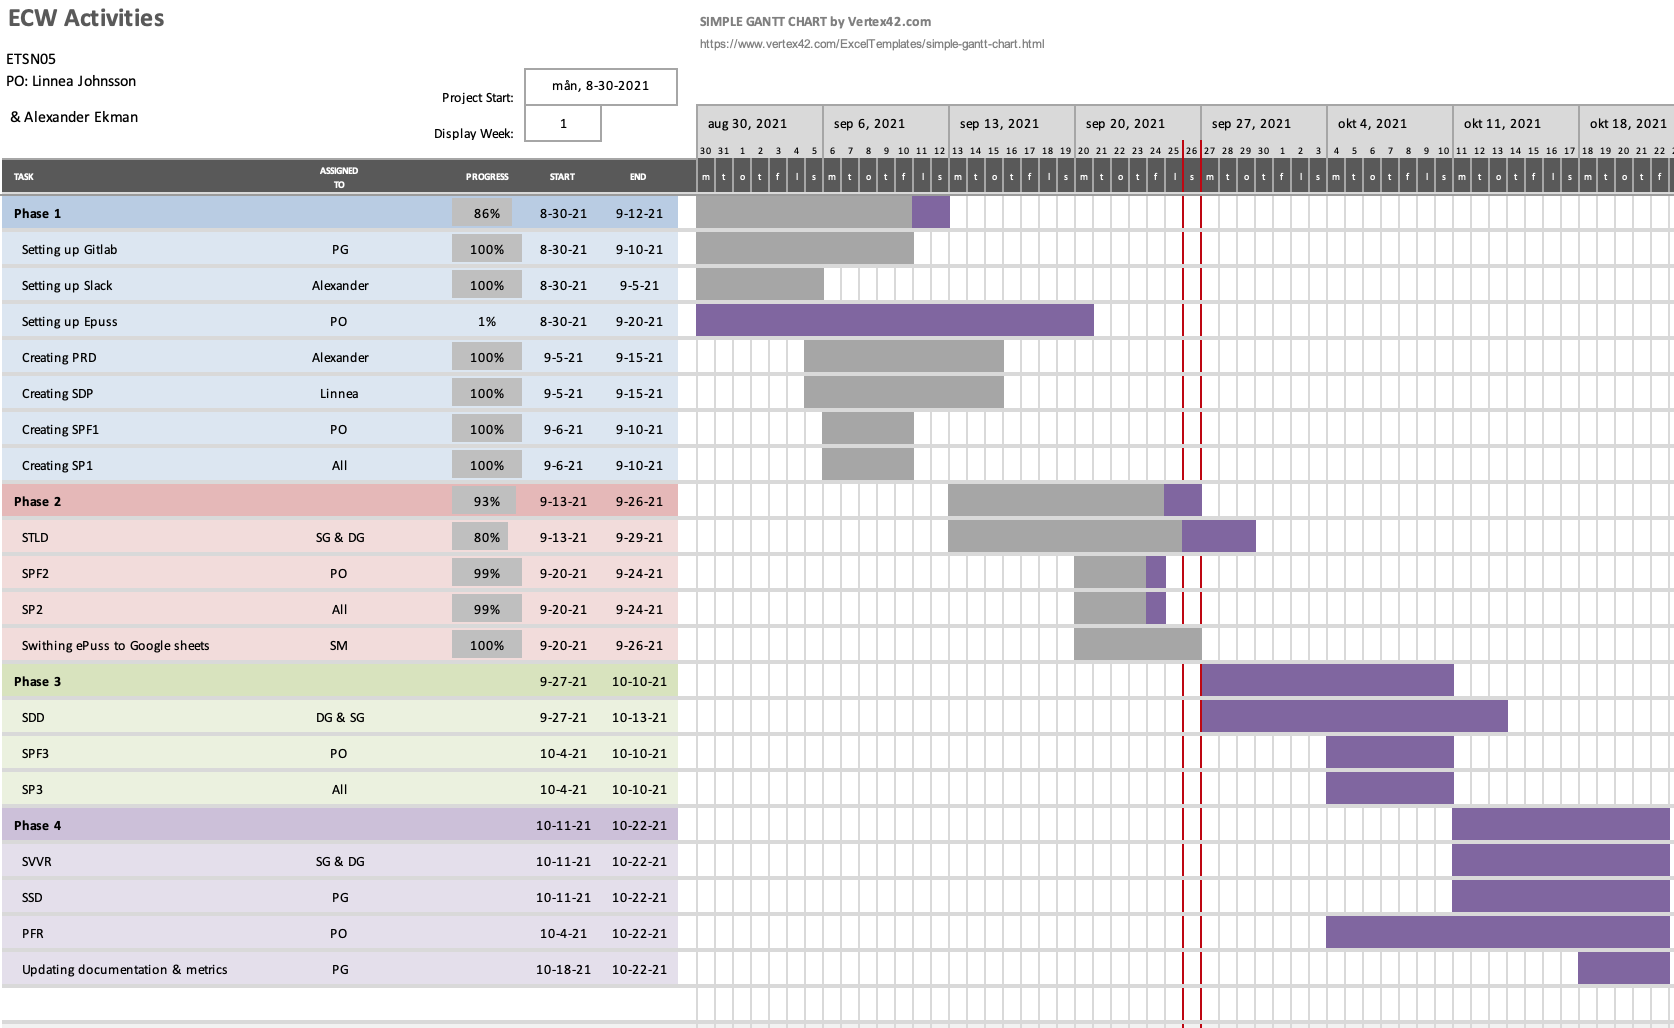
\includegraphics[scale=0.7, angle=90]{sdpFigures/GanttActiV2.png}
    \caption{A time plan represented in a Gantt chart over the main deliverable of the project, besides the code base development.}
    \label{fig:GantAct}
\end{figure}

\subsection{Gantt Development chart}
Gantt charts are also used for the sprint planning. They are used to figure out which issues to start with, and which issues can be carried out in parallel, and which need to be developed sequentially during each sprint. This means that a new Gantt chart is developed for each sprint after the corresponding SPM based on the SFP and SP. 

This decision was made due to the time allocation needed in order to produce a Gantt chart over all issues over all three sprints. Especially when taking into account the time needed to update the Gantt charts to include changes in future plans and the SPF due to missed issues or such when laying out the first plan. Having a detailed plan over issues too far into the future would need a compromise on the agile aspect of the project. The Gantt chart for sprint 1 is presented in figure \ref{fig:GantDev}. 
\begin{figure}[h!]
    \centering
    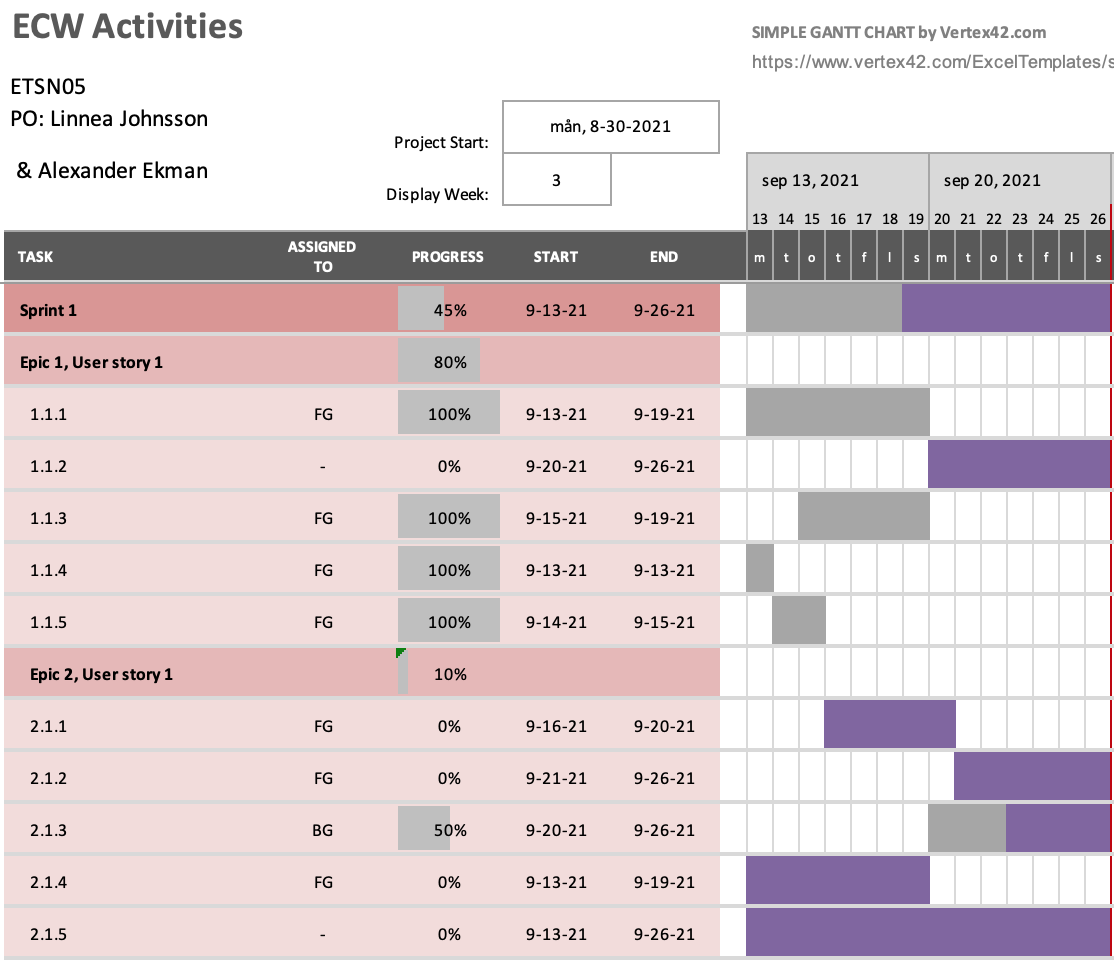
\includegraphics[scale=0.75]{sdpFigures/GanttDevV2.png}
    \caption{A Gantt chart over SP1 as a time plan for development in sprint 1}
    \label{fig:GantDev}
\end{figure}

\section{Time plan follow-up and quality review}
The idea at first was to use the course recommended software EPUSS for time reporting. This plan changed due to information that the software not meeting school requirements. Time reporting will instead be done using a reprogrammed google sheets document where each team member has their own sheet to put in their time spend on different tasks. 

The reported time is tagged with the codes given in the PH section 8, these include codes for working on documentation and meetings. The DG and SG will also use the git command spend when working on issues in order to track their progress. Both of these above mentioned ways of reporting time will then be used to follow up on the time plan and to measure how much we had over- and underestimated.

The follow-up of the time plan is carried out in two more ways. One is measuring the number of pushed up and/or added issues. Pushed up issues refers to issues being moved from one sprint to a later one, either due to time constraints or dependency miss calculations. Added issues instead refers to a user story having more issues added to it after the SPM due to a failure to include sufficient issues to cover the story. The latter can also include one issue being split up into more issues in order to better represent its work load.
Another way to follow up on the time plan is by using a burn down chart and a Gantt chart. These are used in order to easily see the actual progress or time spent in contrast to the plan for each sprint. 

The overall quality of the project is measured in two main ways. The first is measuring how well we estimate and plan the different parts of the projects, i.e. how well we follow the time plan. Secondly, code and deliverables are reviewed in many steps. One of the reviews are made by the SG. This include reviewing developed code before accepting merge requests into the main branch. This is done in order to ensure that the code developed follow the architectural plan of the project. Other, more informal reviews are done continuously both on the code and deliverables by IPMs and EXPs where cooperation and shared knowledge increases the quality. Furthermore, the RevMs provides the team with feedback on the deliverables so that they can be updated and improved before the final hand in, and the final review. 

Finally, the quality of the delivered system is validated and documented in the SSD and SVVR that are produced and handed in during the last phase of the project.

\section{Risk analysis}
The risk analysis presented below was created by using input from the DG and SG. The members gave input from their area of expertise. I.e. they tried to formulate risks based on issues and difficulties they had run into in prior projects. 

\subsection{R1}
\textbf{Description}: Issues being underestimated \newline
\textbf{Likelihood}: 4/5\newline
\textbf{Severity}: 2/5\newline
\textbf{Indication}: More time is spent on issues than planned \newline
\textbf{Prevention}: Basing estimates on experience and not overcrowding the schedule. Split big issues into smaller sub-issues, this makes it easier to estimate each sub-issue correctly. Analyze on sprint retrospective why we overestimated last sprint and avoid to make the same mistake for the upcoming sprint. \newline
\textbf{Damage Control}: Move less prioritized issues to the a later sprint or bring in more developers in order to have more time to allocate \newline

\subsection{R2}
\textbf{Description}: Issues being overestimated \newline
\textbf{Likelihood}: 2/5\newline
\textbf{Severity}: 3/5\newline
\textbf{Indication}: Issues are getting done faster than planed and developers being unnecessarily non allocated \newline
\textbf{Prevention}: Making educated guesses for the estimates and have an updated and prioritized SPF on hand. \newline
\textbf{Damage Control}: Move up more issues from SPF to SP, ask developers if there are bugs needing to be fixed or code to be refactor and allocate the resource to that \newline

\subsection{R3}
\textbf{Description}: Team members getting sick \newline
\textbf{Likelihood}: 4/5\newline
\textbf{Severity}: 2/5\newline
\textbf{Indication}: No good indications, since sickness and other not-planed interference can occur from one day to another, especially in pandemic times. \newline
\textbf{Prevention}: Utilize the digital tools for meetings instead of being in crowded rooms and follow the health departments recommendations \newline
\textbf{Damage Control}: Re-prioritize the SPF and see what can be moved from the current sprint to the next. Use the Scrum Master to help re-organize the work that will not be finished. \newline

\subsection{R4}
\textbf{Description}: Sever bugs appear in phase three \newline
\textbf{Likelihood}: 2/5\newline
\textbf{Severity}: 4/5  \newline
\textbf{Indication}: Little time spent on code review and low-coverage test written, the testing written do not acting as suspected \newline
\textbf{Prevention}: Thorough code reviews and high coverage testings \newline
\textbf{Damage Control}: Cut out affected functionality in order to deliver a functioning system to the final review \newline

\subsection{R5}
\textbf{Description}: Sever bugs not appearing before hand-in \newline
\textbf{Likelihood}: 1/5\newline
\textbf{Severity}: 5/5  \newline
\textbf{Indication}: Little time spent on code review and low-coverage test written \newline
\textbf{Prevention}: Thorough code reviews and high coverage testings \newline
\textbf{Damage Control}: Ask the customer for an extension to bug-fix \newline

\subsection{R6}
\textbf{Description}: Misunderstanding of specifications \newline
\textbf{Likelihood}: 3/5\newline
\textbf{Severity}: 4/5 \newline
\textbf{Indication}: Poor communication with client, long times in between feedback, and ambiguous/vague requirements \newline
\textbf{Prevention}: Ask early-on for clarification, proactively reach out if we find flaws or holes in the current requirements, and/or prototype a solution in the early deliverables and emphasize that we need the customer's feed back on it. Use stand-up meetings to identify any misunderstandings.\newline
\textbf{Damage Control}: Schedule time to refactor current designs, documents, code, and test cases to match the correct specifications while pushing back the development of new functionality. \newline

\subsection{R7}
\textbf{Description}: Miss-scheduling of highly dependant issues \newline
\textbf{Likelihood}: 2/5\newline
\textbf{Severity}: 2/5\newline
\textbf{Indication}: Scheduled issues, for which no progress is made \newline
\textbf{Prevention}: Take extra cation when planning issues that could have high dependencies. Highlight progress of coupled issues on the DSM. \newline
\textbf{Damage Control}: Allocate more resources to the blocking issue and prioritize highly if it is essential for the projects progress. Otherwise push it to a later sprint.  \newline

\subsection{R8}
\textbf{Description}: Conflicting schedules giving meetings low attendance \newline
\textbf{Likelihood}: 3/5\newline
\textbf{Severity}: 1/5\newline
\textbf{Indication}: Few and small windows where meetings can be scheduled \newline
\textbf{Prevention}: Schedule the most important meetings far in advance before the team members schedule fills up. For example plan the most important stand-ups on zoom ahead of time and have the less important stand-ups on slack, where it is easier to attend sometime during the day by text. \newline
\textbf{Damage Control}: Have meeting with few attendees and share the information discussed and action list created with ones missing the meeting. Ask if they have something to ad \newline


\end{document}
